\documentclass[a4paper]{report}

\usepackage[masterthesis,english]{comp}
\usepackage{graphicx}
\usepackage{hyperref}

\title{A General Aspect Orientation Framework}
\author{Chris Vesters}
\principaladviser{Dirk Janssens}
\assistantadviser{Tim Molderez}
\submitdate{May 2014}
\bibfile{references}
\bibpunct{[}{]}{;}{a}{,}{,}

% Make hyperref package use black links
\hypersetup{
	pdfauthor={Chris Vesters},
	pdftitle={A General Aspect Orientation Framework},
	pdfkeywords={Aspect Orientation, Framework},
    colorlinks,
    citecolor=black,
    filecolor=black,
    linkcolor=black,
    urlcolor=black
}

\begin{document}
\frontpages

\clearpage 
\phantomsection 
\addcontentsline{toc}{chapter}{Nederlandstalige Samenvatting}
\chapter*{Nederlandstalige Samenvatting}

\clearpage 
\phantomsection 
\addcontentsline{toc}{chapter}{Acknowledgements}
\chapter*{Acknowledgements}

\clearpage 
\phantomsection 
\addcontentsline{toc}{chapter}{Abstract}
\chapter*{Abstract}

\mainbodypages

\chapter{Introduction}
\section{Aspect Oriented Programming}
Aspect oriented programming (from now on referred to as AOP) is a way of programming that allows separating code beyond the capabilities of object oriented programming. It allows the separation of cross cutting concerns from the core concerns, by doing this we achieve more modular code, prevent code tangling and code scattering which results in code that is easier to maintain and modify.
\begin{figure}[h!]
\centering
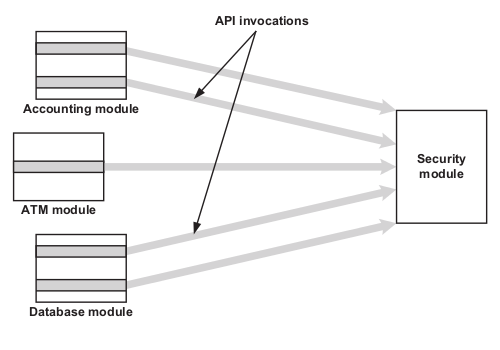
\includegraphics[scale=0.5]{images/Code_Scattering.png}
\label{fig:Code_Scattering}
\caption{A representation of code scattering\cite{Laddad10}.}
\end{figure}\\
\begin{figure}[h!]
\centering
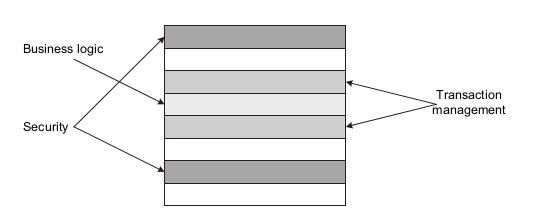
\includegraphics[scale=0.5]{images/Code_Tangling.png}
\label{fig:Code_Tangling}
\caption{A representation of code tangling\cite{Laddad10}.}
\end{figure}\\
AOP works by identifying join points, which is certain point in the execution of the program. The set of all the join points is called the join point model. It is at these join points that we can modify the original program execution. This change can go from something as simple as logging to something more invasive where the original code isn't even executed at all.\\
A first thing we need is a way to indicate which join points we want to work on, this is done by a point cut. Now we can refer to certain join points we also need a way to modify the execution. This is done by an advice, note that there can be multiple kinds of advice.\\
In the end everything has to come together, this is done by the weaver.\\
\\
The most known AOP language by far is AspectJ, which is an extension of Java. To demonstrate the concept of AOP a couple of AspectJ examples are shown here:\\
TODO: EXAMPLES!\\

\section{Problem}
Currently AOP is often implemented by extending an existing language, this often leads to completely new languages requiring new compilers and  breaking existing tools for the base language. Especially the latter is a reason why some people haven't made the step to start working with aspect oriented languages.\\
\\
Though the concepts of AOP are quite general, which is reflected by the similarities in different aspect oriented languages, all the AOP parts of these languages were written from scratch. The main reason for this is the absence of a general language independent library or framework to handle aspect orientation. Another reasons is that by building a language from scratch you get more freedom to implement the desired features.

\section{Goal}
The goal of this thesis is to build a framework that encloses all core ideas of AOP in an abstract manner without being specific about a particular base language. This will enable use to use the framework to develop an aspect oriented language quicker and easier than currently is the case by extending a couple of parts. The framework will work for completely new languages, and existing ones we want to extend. The latter one will pose the most problems as the freedom to adapt the compiler is very limited. (TODO: add in a later section the idea of injecting the code into a compiler with AspectJ)

\chapter{Aspect Oriented Language Components}
An aspect oriented language consists of several components, to explain these I will start from the base language and work my way up to get an aspect oriented language. At every point I'll make it more concrete with a small AspectJ example.\\
\\
The starting point of creating an aspect oriented language is the base language, this is the language that we want to extend or is a completely new language. In the latter case the base language will be the new language excluding all the aspect oriented features. The base language can be any kind of language: procedural, object oriented, functional, logical, data oriented, ... (TODO: EXAMPLE)\\
\\
By defining the base language we implicitly defined a join point model. This is because the join point model consists of all the points that occur during execution on which intervention of the aspects is allowed. The join point model will always remain implicit, but it is an important part of any aspect oriented language as it is the link between the base language and the aspect oriented part.\\
\\
Knowing at which points we can intervene doesn't allow us to do anything, we need a way to identify certain points. This identification is done by using pointcuts, specifying one or more join points. They way in which pointcuts allow us to refer to join points should be as close as possible as the way in which they appear in the base language. (TODO: EXAMPLE)\\
\\
Now that we can refer to certain join points, we can actually start modifying the original code. This modification is encapsulated in an advice, which contains 'code' that has to be executed. When this 'code' is executed is defined by the pointcut with which the advice is associated. Whenever the program passes a join point that matches with the associated pointcut, this advice must be executed. The 'code' in the advice should be written in the base language to prevent the user from learning an entire new language. (TODO: EXAMPLE) The advice should also be able to have access to information about the join point, this information will be provided by the pointcut.\\
\\
One problem that arises is: what is suppose to happen if we encounter a join point at which multiple advices are to be executed? This can be either caused by multiple pointcuts matching to the join point, or multiple advices being associated with the same pointcut. The latter case can be easily solved as we can combine the two advices into one bigger advice. The first is a bit more tricky since the one pointcut can also match other join points, different from the other, which means we can't just combine them. (TODO: illustrate) The solution to this is of course to introduce an ordering mechanism. This ordering can be either placed on the pointcuts or on the advices, in the first case we still need to make sure that there is only one advice for each pointcut though.\\
\\
One final component we need, is something that will actually make sure that the advices are executed when the join points are encountered. The weaver will make this happen, and can do this in multiple ways. The easiest is compile-time, weaving which comes down to a pre-processing step, a more advanced form is run-time weaving, yet other forms are available depending on the base language. (TODO: EXAMPLE)\\
\\
With the components specified above we are perfectly possible to create an aspect oriented language, despite that we note that some features are still missing, as an example we note that communication between different advices is impossible. Since aspect orientation is often presented as an extension of object oriented programming it makes sense to introduce some form of class, called aspects. These aspects will contain the advices, which match functions and methods in object oriented languages, and can be extended to have members too. By doing this we immediately have can provide the advantages offered by object oriented languages among which are inheritance and encapsulation. (TODO: EXAMPLE)\\
\\
An overview of all the components and how they are linked together is shown in figure (TODO:REF). The weaver is not considered to be part of the aspect language just as a compiler is not considered a part of the language.

\chapter{Aspect Oriented Framework}
Since the framework has the be easily extensible to work with any kind of language it has to be very abstract and may not contain any information about a base language. On the other hand, creating a framework that is too abstract and general requires too many additions to be made to implement it for a base language, making the framework completely missing its goal. The level of abstraction has to be well considered.\\
\\
I will first go into detail how the components that were identified in the previous chapter are represented and work in the framework. The explanation of the weaver is preceded by some information that is required to fully understand how the weaver works. This is followed by some remarks about the current version of the framework, and to conclude the chapter I explain how we can now expand this framework to work with any base language.\\
\\
The first component of the aspect language that we identified were the pointcuts. This component is implemented as an abstract class Pointcut, to completely specify a join point we need some way to identify it's signature, this however is language specific and can therefore not be provided by the framework. Other common structures are arguments and context. The arguments are meant for information that can be used in the advice, while the context is a way to restrict matching join points based on  information that goes beyond the scope of the join point.\\
\\
Something we notice, which is also the case for AspectJ, is that it is not possible to identify completely different join points with one pointcut. This complicates writing advice that has to be executed on these two different sets of join points. To simplify this we allow grouping pointcuts into sets, this is implemented as a PointcutSet, which has a set of pointcuts, arguments that are available for the advice, and should be present in all the poincuts of the set, and a name so we can link the advice to this pointcut. (TODO: add diagram)\\
\\
The advices are implemented by the abstract Advice class. This class has a name (String), which will make ordering them a lot easier, and a set of arguments (Argument), these arguments are the ones that can be used inside the advice body. Note that the arguments of the pointcut to which this advice is linked must be assignable to these arguments. The body or actual code of the advice is not provided by this class, simply because it depends on the base language as we want this to be in the same formalism. (TODO: add diagram)\\
\\
Before going any further some more explanation about some already mentioned concepts is required. I have talked about arguments and a context, but didn't mention what these are. A context is the easiest, since  the context can be anything and highly depends on the base language the only thing the framework provides is an interface Context. An argument is a bit harder, every base language has its own vision of what an argument is, though two concepts are very common, being a name and a type. For this reason the Argument class has a name, which is also required for access to the argument and a type. The type however can not be a base language type, but should be more general. For this reason an interface called Type was created.\\
\\
This being said we can now discuss the remaining components being: the order mechanism, the aspect and the weaver. The components will be handled in the order they are specified here.\\
\\
The framework does not provide a basis for the ordering. This means that the user is free to implement the way of specifying an ordering as he likes. The user is also free to choose whether the order will be specified on the pointcuts or on the advice. Despite the freedom on the ordering 'language' the ordering itself is still limited. This will be discussed into more detail once the weaver is introduced.\\
\\
The current version of the framework does not provide any concept of 'aspects', though this causes some limitations, it does not make the framework useless. Some of the limitations were already mentioned in the previous chapter, more details about the consequences of the absence of an encapsulating aspect is discussed at the end of this chapter.\\
\\
Before discussing the weaver we have to make some things a bit clearer. You might be wondering how the join points will be extracted from the source code. This is done by the parser of the base language, or a modification of it. The join points that are generated by this parser will actually be instances of the Pointcut class. By doing this comparing whether a pointcut set contains a pointcut that matches the joinpoint becomes trivial.\\
\\
Something you might have noticed is that the advice does not keep a link to the pointcut itself, nor the other way around. The link between pointcut and advices is handled by the weaver, this allows a better separation between pointcuts and advices and gives the weaver more freedom to operate.\\
\\
The ordering mechanism requires some extra information as well, I mentioned earlier that despite the freedom some limitations still exist. This is cause by the way the weaver handles the ordering internally. The weaver will keep a list for every advice to its preceding advices. This means that the ordering provided to the weaver has to be on the advices, and should result in a partial ordering (TODO: add image)\\
\\
A final remark that has to be made is how the framework handles the argument mapping from adivce to pointcut and join point. For this the framework provides a Match class that contains a map from one argument to another. (TODO: add image) This allows us to specify a mapping between arguments, which will be used to eventually translate the arguments of an advice to that of the join point.\\
\\
This brings us to the last component, the weaver. Just like most elements in the framework is the weaver implemented as an abstract class. This abstract class provides a way for all components to register their information, which is then stored to be processed. They way in which the information can be processed depends both on the base language and the possibilities of the base language parser and can therefor not be implemented by the framework. The framework does however provide a way to specify the input and output files by using flags, an overview of these flags can be seen in (TODO:REF).
\begin{table}[h]
\centering
\begin{tabular}{l l}
-a \textit{files} & Specify the aspect files.\\ [2ex]
-s \textit{files} & Specify the source files.\\ [2ex]
-oDir \textit{dir} & Specify an output directory (optionally).\\
\end{tabular}
\caption[tab:Flags]{An overview of the flags available in the weaver.}
\label{tab:Flags}
\end{table}\\
Besides that it also provides some methods that simplify processing the information. The most important one is 'executingAdvices', given a certain joinpoint this method will return all the advices that have to be executed in the order they are returned. In case the user needs to know the pointcuts that match a certain joinpoint a method 'enclosingPointcuts' is provided. The framework also implements a way to compare advices based on the partial ordering, this is done by the AdviceComparator which is an extension of the Comparator. This is meant for internal usage and the user should not need to use this since the return value of the 'executingAdvices' method is already ordered. (TODO: add image)\\
\\
A complete overview of the framework and how everything is connected can be seen in figure (TODO: REF).\\
TODO: add image\\
TODO: some remarks about this?\\
\\
Some trade offs had to be made when designing the framework, it are these trade off that I now discuss into more detail. First of all it needs to be noted that both Context and Type are interfaces which both specify only one method called 'isAssignable'. This means that Context and Type, though called different, do the same thing. We could use one general interface, this is not done though to be able to handle future evolution.\\
\\
Adding a notion of aspect would allow a lot of nice features such as adding members that can be used for communication between advice and inheritance. They could also be used as a way to encapsulate pointcuts and advice, though this can also be done without aspects simply by separating them over multiple files.\\
Adding aspects to the framework would have introduced a lot of extra complexity. Since the goal of this thesis is to demonstrate the usability of such a framework I have chosen to not include this, but keep it as a future work.\\
\\
The framework uses an abstract notion of type, this is to achieve the level abstraction required to separate the framework from the base language. This however means that for each base language we need a new type system that implements the Type interface, which might result in a lot of work. Sometimes it is however possible to use the same type system the compiler of the base language uses if we can add the interface to it.\\
\\
The advice and pointcuts are not directly connected with each other, the connection is achieved by the weaver. Because adding an explicit link does not provide any advantages, I have chosen to do it this way to ensure that the components are as loosely coupled as possible. Nevertheless the framework demands that at the moment a pointcut is added the pointcut set it is linked with must be be known to the compiler.\\
\\
Something that was not discussed so far is what happens if a join point is encountered that is matched by multiple pointcuts in the same pointcut set. In this case there basically are two options: either we execute the advices for each matched pointcut, or we only select the first matched pointcut of the set. Currently the latter is implemented in the framework, mostly because if we still want the first to happen, we can simply split the pointcut set.\\
\\
One final remark that has to be made is that implementing both join points and poincuts as the same Class can be dangerous since they are not the same. One example is that poincuts can contain wildcards wile join points should not. It may also be feasible to allow specifying types and sub-types in pointcuts, where in the join point the types are fixed and known. This means that we have to use the Poincut class carefully if we use it with a join point.\\
\\
(TODO: can we ommit the context type and just add all this stuff as arguments?)\\
\\
To conclude this chapter I will briefly explain how the framework can be expanded to work with a base language, for more detailed examples I refer to chapters (TODO: REF) where the framework is expanded for two different languages. Before being able to use the framework you have to specify a language in which it is possible to specify pointcuts, advice and optionally an order. You have to provide a parser for this language, it is this parser that will create the pointcuts and advices which are handed over to the weaver.\\
\\
The pointcuts and advice that has to be created has to be specific for the base language, this means that you first have to create a subclass of Advice and one or more subclasses for Pointcut.
The advice subclass is simple, it must contain the body of the advice. The pointcuts need to contain all information to identify a join point. Since there will be multiple types of pointcuts you will have to implement one subclass for each type of pointcut. If you desire to add a context to the pointcut, you still have to create a class with the Context interface that contains all the context information you want to use.\\
\\
The pointcuts and advices ofcourse require you to implement a type system. Depending on the availability of the type system used by the base language, and more precise the compiler, it is possible to add small modifications to get the type system without much work. If not, this might be a bigger problem.\\
\\
Now you can create pointcuts and advice you still need to expand the Weaver class to add the actual weaving. Since the framework gives you the advices to execute for each join point all the extended weaver has to do is execute these advices at those times. This sounds easier than it sometimes is though, especially the way of how you can interact with the base language is important. (TODO: overview of interaction between languages and weaver)\\
\\
I know this sounds vague and very abstract, which is why I refer to chapters (REF) again since they contain worked out examples.\\

TODO: explain how to extend the framework!\\
\\
\\
// Old version:\\
The constructed framework provides a basis for all compontents using several classes such as Pointcut, PointcutRule, Context, Advice and Weaver. (TODO: change names of Pointcut to PointcutSet and PointcutRule to Pointcut) (TODO: Add class diagram!)\\
\\
A pointcut can have multiple rules, it are these rules that will match with a join point. To easily compare these rules and a join point, both are specified in the same way (as a PointcutRule). Though this results in situations where we have to be careful.\\
\\
To supply global information to a PointcutRule, we can provide it with a Context. The most common use of such a context is to provide a call sequence.\\
\\
Languages can be created as you like, which is a good thing, because they should be similar to the base language. Though, the result of the languages are extensions of the abstract PointcutRule and Advice class.\\
\\
You can specify an order as you like, but it eventually should come down to a partial ordering, which the framework can handle.\\
\\
Though it is possible to work with an ordering on the pointcuts, the framework works with an ordering on the advice. This allows more flexibility and is in general easier to understand.\\
\\
What is still required to add support for aspect-oriented constructs to a language?
\begin{itemize}
\item Specify a language for the pointcuts and advices. Since these languages should be as close as possible to the base language, the framework can not provide these for you.
\item Extend the abstract class PointcutRule, based on the join point model which is specific to the base language. You have to provide one extension for each kind of join point. The extension however is limited to adding the required information and a method 'encloses' to specify whether one pointcut encloses another.
\item Extend the abstract class Advice, this extension is required to put the body that should be executed in the advice. Since this body will be specified in the base language or something very similar.
\item Extend the abstract class Context, to add all global information that you want to use in your poincuts. This is not required though, but can be used to extend the expressiveness of the language.
\end{itemize} 
Since the framework is separated from the syntactical elements you need to create a language to specify aspects, pointcuts and order. It are these pointcuts, aspects and order that you have to pass to the weaver. These languages are often created from scratch, which means you can take AOP into account when designing the parser. The parser for the base language however may already exist, and a lot harder to modify. Nevertheless should this parser be changed such that it can extract join points from the code and provide these to the weaver.\\
\\
Though it is possible to use different languages for pointcuts, aspects and order, I have chosen to use one language to specify it all. The main reason for this is that there is a high dependency between the components and some similarities. By using only one language I can exploit the similarities and minimize the amount of work required.

\chapter{Small C}
\section{Introduction}
Small C is a minimal subset of the C language. It does not support structs or including other files, though printf and scanf are supported. There are two reasons why this language is chosen, it is a small language that still contains the elements of modern day programming languages and a compiler was available and modifiable.\\
\\
TODO: EXAMPLE OF SMALL C

\section{Aspect Orientation}
The join point model consists of calling and executing functions and getting and setting the value of global variables. This means that there are two sub-classes of PointcutRule, being MethodPointcutRule and MemberPointcutRule.\\
Because there is no context provided the join points for a function call and a function execution will give the same result. The distinction is however made to show it's potential usability.\\
\\
There are three advice kinds for executing a function advice: before, around and after. It would be possible to only allow around advices since before and after are special cases. For the variable advice there are only two moments: before and after.\\
\\
You can specify an order of executing the advices since conflicts may arise. This order is specified explicitly by saying that one advice is 'bigger' than another. The result of this order is that the biggest advice 'encloses' the smaller one.\\
TODO: show it with an image.

We notice that the order for an after-after conflict is the inverse of that in a before-before conflict. This may seem weird at first, but the reason for this is that we need to be able to resolve around-around conflicts. In this case we want one around advice to enclose the other, this however means that the before part of this enclosing advice comes before the other advice, but the after part comes after it.\\
\\
TODO: explain how the file changes: wrappers!
\section{Examples}
TODO

\section{Difficulties}
Despite having a modifiable compiler, there were a lot of problems of weaving the advices into the code. This was caused by the fact that the compiler was not designed to allow changes after parsing the code. Changing this would require big changes in the compiler and was therefor not really an option. Instead of changing the compiler another alternative was used, by creating two compilers, both with small changes, we could weave the file in multiple passes.\\
\\
In phase 1 the source code will be parsed and all join points will be specified to the weaver. The weaver will produce wrappers and add these to a temporary output file. In phase 2 the modified file will be parsed and the original calls will be modified to point to the wrappers. In phase 3 the actual advice bodies will be written to the wrappers. Phase 4 is to compile the weaved file with a regular compiler, this is not done by the weaver and has to be done by the user himself.\\
\\
It was impossible to change the calls in the first phase due to a simple circular dependency. The compiler checks that the called function actually exists. Since the compiler does not allow to add declarations before the current point, these declarations have to exist in the source code itself. To do this however we need to know which join points occur, and thus we need to have parsed the file before.\\
\\
Adding the content can not be done before phase 2, simply because the content contains function calls to the actual functions which need to be kept. It is impossible to distinguish a call from within a wrapper from one within a 'normal' function, yet we need to treat them separately. Therefor we need to add the content in a separate phase.

\chapter{Dot}
\section{Introduction}
Dot is a language that allows you to easily specifies the structure and appearance of a graph. The features it supports are directed edges, undirected edges, subgraphs, labels for nodes and edges, different shapes, colors and more.\\
\\
Because there is no time aspect related to dot, adding AOP may seem weird since join points are defined as points in the execution of a program. This actually means that the join points simply map to points in the code in a static way. Yet the ideas of AOP can still be applied.\\
\\
TODO: EXAMPLE OF DOT

\section{Aspect Orientation}
The join point model consists of nodes and edges, for which we can specify required attributes, and graphs, which is used to specify pieces larger than one element. To achieve this there are three subclasses of PointcutRule: NodePointcutRule, EdgePointcutRule and GraphPointcutRule.\\
\\
An advice may consist of attributes (for nodes or edges) and/or entire nodes or edges in the case of a graph pointcut. For each advice you need to specify what to do with the elements, you can either add them or delete them. Because there is no notion of time, you don't need to specify when the advice should be executed.\\
\\
Despite the absence of time, you may still need to specify an order when advices operate on the same elements. In such cases changing the order may lead to different results.

\section{Examples}
TODO

\section{Difficulties}
The biggest problem encountered was how to decide on the syntax of the Aspect Orientation Language. Once this was done adding Aspect Orientation went really fast, also thanks to the compiler which allowed it to easily modify the graph and write it back to file.\\


\chapter{...}
- Introduction to base language.\\
- Pointcuts + Other Aspect Oriented related stuff.\\
- Difficulties.
\chapter{Discussion}
- To what extent are parts being reused? (or not)\\
- How much coupling is there between the base language and the module?\\
- How flexible is the model? What range of base languages can it handle?
\chapter{Future Work}
- Add the concept of 'Aspects', this will be similar to Objects in an OO language.\\
- Add global variables, is this useful? We will need a general wrapper.\\
- It should be easier to use it on run-time.\\
- Debugging isn't really possible -> keep links from the weaved to the original code.\\
- Optimizing the weaving process, currently each change will require to completely re-weave all the code.\\
\chapter{Related Work}
- About building languages from modules in general .. or about building languages out of smaller languages (also called language composition)
\chapter{Conclusion}

\chapter{Temporary Stuff About Languages}
It is impossible to keep on implementing more and more languages. Therefor I will discuss existing aspect oriented languages and how they could be implemented using the framework.
\section{AOWP}


TODO: REFERENCE!\\
As mentioned in the paper, we need to provide a context to be able to handle coming from a certain page. This can be done by adding this information to the context of the pointcut and join point. The paper mentions different events the language can handle, if the language were to be made with the framework we would have to create a PoincutRule for each of these events (or divide them into groups!).\\
\\
The framework does not provide the '\&' or '!' operator, only the '|' is available by specifying multiple pointcutrules in one poincut. Though it is an inconvience, it is not a big problem since we can create an AndPointcutRule which simply takes two other pointcutrules and matches if both match. The same goes for the NotPointcutRule which will invert the result of a pointcutRule.\\
\\
In it's current form the framework does not provide run-time weaving. It is however to solve this problem in two different ways. The first is by adding extra code that checks the run-time information and makes a decision based on that. The second is by calling the weaver at run time.  By doing this the run-time information is available at the moment of weaving and can be used to specify pointcuts.\\
\\
Since the framework lets the user specify a languages as he likes, the same language can be used as in the paper as long as there is a compiler for it.
\section{AspectGrid}
TODO: REFERENCE!\\
Since it is required to design your own aspect langauge, we can design it that way that the details are hidden as is mentioned in the paper.\\
AspectGrid itself is based on AspectJ, which makes creating it pretty fast and easy. The framework presented here in this thesis is more general and does not provide existing pointcuts. This means that using this framework instead of extending AspectJ takes a bit more effort.\\
\\
It is however perfectly possible and it will share many resemblances with the Aspect Oriented version of Small C that was earlier presented in this thesis. The reason for this is that AspectGrid focuses on spreading computational load, and will therefor focus on the function calls, other pointcuts such as getting and setting a member aren't relevant.
\section{AspectMatlab}
TODO: REFERENCE!\\
To add extra information to the pointcuts as is done in the paper, we have to add members to the specific subclasses of the PointcutRule.\\
\\
Pointcuts are: call and execution of methods, get and set of arrays and a special loop pointcut. The within will not be part of the PointcutRule but will be provided as a context.\\
\\
The translation to matlab code can be done the same way with the framework as it was done in the paper.\\
\\
AspectMatlab orders the pointcuts implicitly, the designed framwork does not do this. This means that to maintain the implicit ordering caused by the order of appearance we need to add an explicit ordering to the pointcuts during parsing.\\
\\
The context selectors add contexts to the pointcut or advice (DON'T UNDERSTAND! LOOK IT UP!!!) which can be done by using the context for PointcutRules.\\
\\
The designed framework does not provide a way to share information between advices, or even between the same advices that is run multiple times. To achieve this we have to rely on the options present in the base language. (LOOK UP: is there static stuff in matlab?!)
\section{Conspects}
TODO: REFERENCE!\\
REREAD THIS, it doesn't make much sense!\\
\\
To be able to work with the framework we need to shift a lot of things, first we note that the contexts as presented in the paper can not be achieved. This is however not really a problem since they can be implemented as plain Java Classes.\\
The idea of the event methods that are presented in the paper match what the framework considers a pointcut, there are however some differences. The framework does not allow code in pointcuts in contrary to event methods. The optional guard that can be added will result in a context for the pointcutrule.\\
\\
There seem to be an explicit invocation of events, this can not be done with the framework, and I need to look into this a bit more.\\
There seem to be no real pointcuts, they are part of the advice. This will not be a problem for the framework.
\section{DISL}
The open joinpoint model can be implemented by having a general pointcut to represent a set of byte code instructions. It's up to the parser to detect these sets of byte code.\\
\\
Compatibility with Java and the Java virtual machine is in my opinion achievable since the framework is written in Java. If we look at the more general idea of compatibility we may encounter some problems that are hard to fix and require some workarounds.\\
\\
Access to context data can easily be provided by adding it to the join point and at the same time we can check on this data by setting it in the point cut as a kind of guard. Allowing the user to define its own context elements is harder. How we can do this is not clear, let me think about it.\\
To add the dynamic information it is best to run the weaver at run time.\\
\\
Instrumentations map to advice.\\
Markers map to pointcuts.\\
To add custom markers the weaver needs to be able to detect them, how are we going to do this? Let me think about it.\\
\\
The order is based on numbers: these need to be turned into an partial order, but that's easy.\\
Also, the implicit order of appearance has to be made explicit to the weaver. The parser can do this by making an order while parsing where he states that the previous encountered one must occur before the next encountered.\\
\\
The communication between snippets may be a problem.\\
Static \& Dynamic information: try to hack it in -> We can just do this! (Or what is meant with this?)\\
Guards \& Scope: add context to pointcuts (or part of pointcuts itself). It can be used as a guard if the pointcut has filled in information.
\section{KALA}
TPMonitor => Specify Outside of framework? => Communication?\\
\\
Actions of transaction depend on run-time. (TPMonitor guards this => determines what to do)\\
Secundary transaction: requires check at run-time.\\
\\
KALA declaration = pointcut, no names are used (pointcut needs to have name -> add it while parsing).\\
The extra properties declared inside it are the advice.\\
Framework requires splitting them, but this can be done implicit by the parser.\\
\\
Framework doesn't care about content of advice, that's up to the parser. This makes nested blocks possible.\\
\\
Translating code to work with TPMonitor can be done.\\
Using Reflex will become impossible, but the idea remains the same.\\

\backpages
\begin{appendices}
\chapter{An appendix}
\label{chapt:appendix}

\end{appendices}

%\begin{thebibliography}{9}
%\bibitem{Laddad10}
%  Ramnivas Laddad,
%  \emph{AspectJ In Action}.
%  Manning Publications, Greenwich,
%  2nd Edition,
%  2010
%
%\bibitem{AOWP}
%  
%  Aspect-oriented Programming for Web Controller Layer
%Keiji Hokamura
%Naoyasu Ubayashi
%Shin Nakajima
%Akihito Iwai
%\end{thebibliography}

\end{document}